\begin{figure*}[]
\caption{DiffTrace Overview}
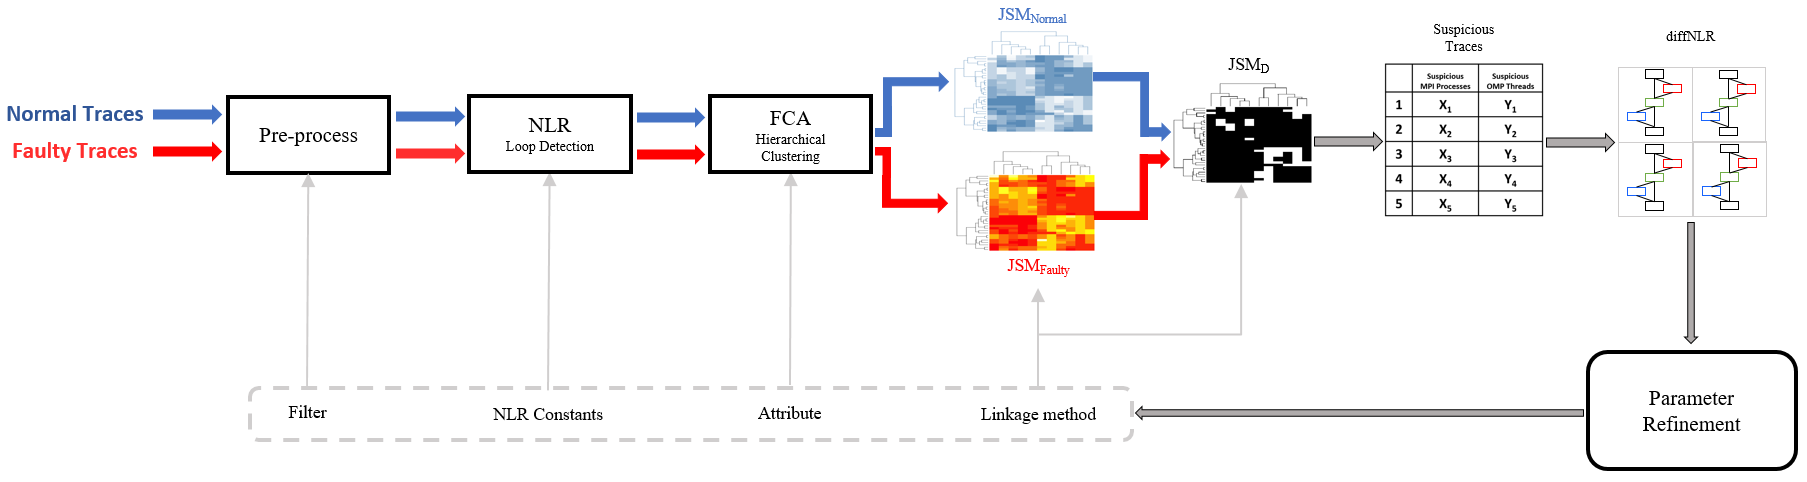
\includegraphics[width=0.95\textwidth]{figs/overview.png}
%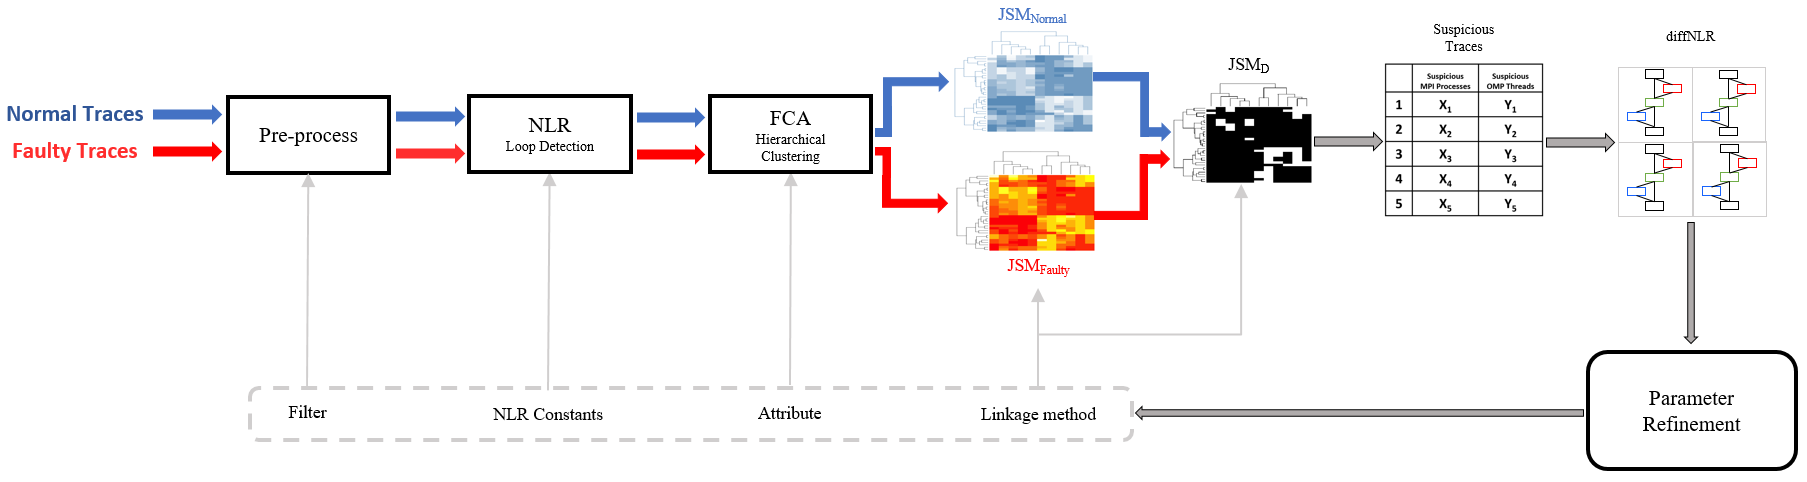
\includegraphics[]{figs/overview.png}
%\includegraphics[]{figs/overv}
\label{fig.diffTraceOverview}
\end{figure*}

DiffTrace employs
ParLOT's~\cite{parlot} whole-program function-call and return trace collection
mechanisms, where ParLOT captures traces
via Pin~\cite{pin} and incrementally compresses them using our trainable
compression schemes~\cite{martin-compression-paper}.
%
ParLoT can capture functions at two levels:
the \textit{main image} (which does not include library code)
and \textit{all images} (including all application code).
%
As the application runs,
ParLOT generates per-thread trace files that
contain the compressed sequence of the IDs of the executed functions.
%
The compression mechanism is light-weight yet effective,
thus not only reducing the required bandwidth and storage but also the
runtime relative to not compressing the traces.
As a result, ParLOT can capture whole-program traces at low overhead
while leaving the majority of the disk bandwidth to the application. 
%
Using whole-program traces substantially reduces the number of overall
debug iterations because it allows us to repeatedly analyze the
traces offline with different filters.


The DiffTrace tool-chain (Figure \ref{fig.diffTraceOverview}) provides

A fault may get triggered at some point in the code and be immediately visible, or it may only manifest itself some time later.



\begin{figure}[]
\centering
\caption{Simplified MPI implementation of Odd/Even Sort}
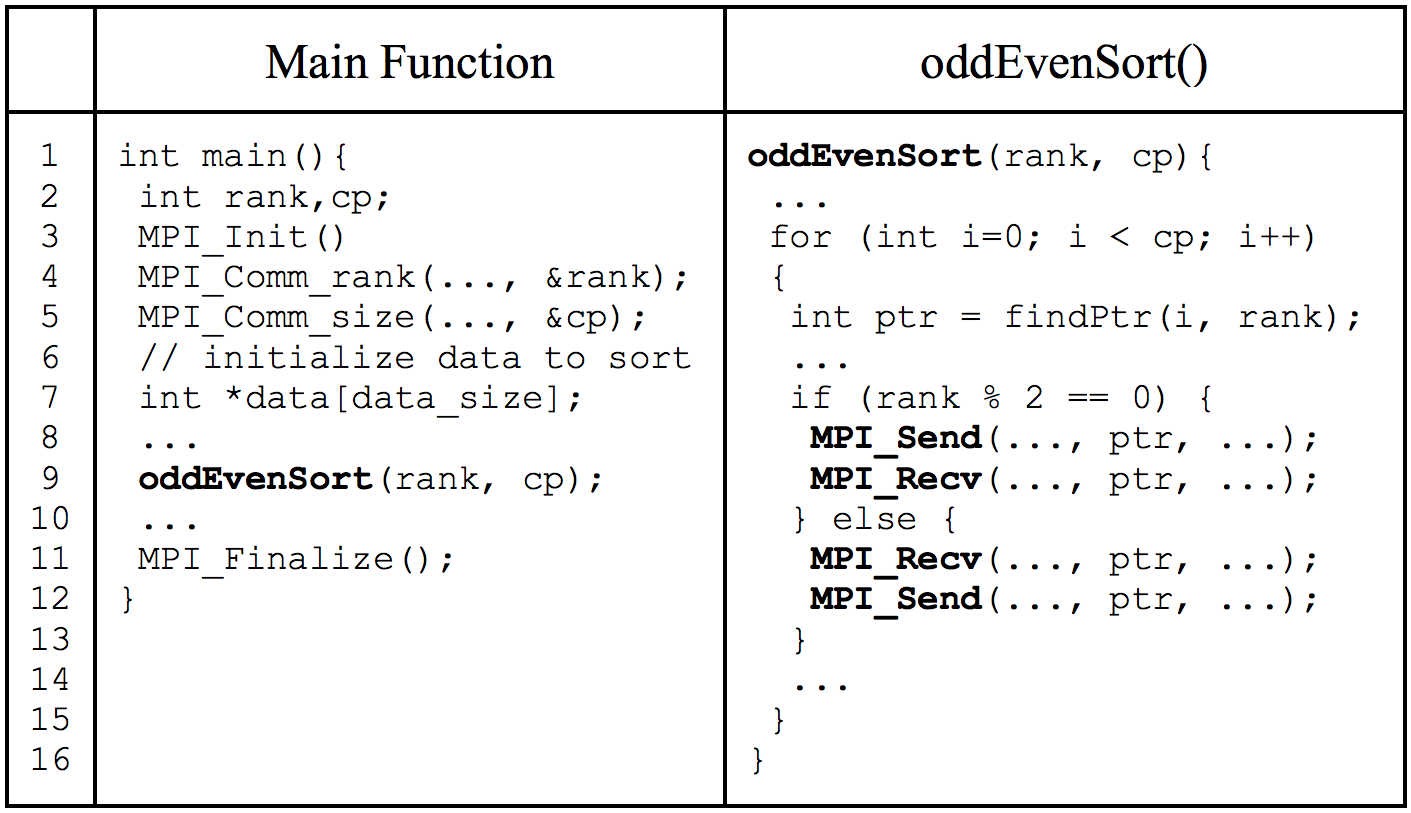
\includegraphics[width=0.45\textwidth]{figs/oddEven.png}
\label{fig.oddEven}
\end{figure}

DiffTrace starts by \textit{pre-processing} the traces. ParLOT traces are highly compressed and typically contain functions that are not of interest to the current analysis. Thus, DiffTrace first decompresses and prunes the traces.
%
Loops appear as \textit{repetitive patterns}, resulting in often long but redundant trace information. A ``nested loop recognition'' mechanism then extracts the loops from the traces. The resulting information not only serves as a lossless abstraction to ease the rest of the trace analysis but also as a per-thread ``\textit{measure of progress}''.
%
The control flow in parallel programs often follows a \textit{specific pattern} such as SPMD, odd-even, or master/slave \cite{?}. As a consequence, the traces of a single execution tend to fall into just \textit{a few} ``equivalence classes''. 
%
%Adapted from the work by Webber et al \cite{weberStructural}, we have applied \textit{formal concept analysis} (FCA)\cite{clbook} techniques to reduce the trace search space into a few classes of traces, and also using the \textit{concept lattice} (CL) data structure as the \textit{model} of execution for further analysis.
%
\hl{definition of ``fault'' maybe? a software bug, node failure, a library version update or porting to a new system that causes failure to a working software }
To study the impact of a fault on the execution, DiffTrace classifies the collected traces and measures the \textit{similarity} between the equivalence classes from the faulty and the fault-free execution.
%
The basic idea is to find out which traces (and, consequently, processes/threads) are falling into a different class (i.e., cluster) when the fault is introduced.
%
Based on the observed similarity among the two clusterings, DiffTrace suggests the topmost suspicious traces, i.e., the traces that suffer the most from the fault, for deeper analysis.
%

The rest of this section illustrates the DiffTrace components on sets of ParLOT traces from the aforementioned MPI odd/even sort example (Figure \ref{fig.oddEven}).
Odd/even sort is a parallel version of bubble sort and operates in two alternating phases: in the \textit{even phase}, the even processes exchange (conditionally swap) values with their right neighbors, and in the \textit{odd phase}, the odd processes exchange values with their right neighbors. The for loop in line 4 of \texttt{oddEvenSort()} iterates over the phases of the algorithm. Based on the phase, the appropriate partner for each rank is computed by the function \texttt{findPtr()} (line 6). The odd/even ranks then exchange their chunks of data (lines 9-13) and sort, merge, and copy operations are performed on the received data (denoted by \texttt{...} in line 15 for simplicity).

According to the MPI standard, \texttt{MPI\_Send} may \textit{block}, meaning MPI may buffer the outgoing message, in which case the send call completes before a matching receive is invoked, or it may choose not to buffer the message. In the latter case, the send call will not complete until a matching receive has been posted and the data has been transferred to the receiver. So, based on the dynamic behavior, swapping the statements on lines 11 and 12 of Figure \ref{fig.oddEvenDL} might end up causing a deadlock. DiffTrace can extract evidence from the traces to locate the cause of such deadlocks and other faults.

\subsection{Pre-processing}
% Please add the following required packages to your document preamble:
% \usepackage{multirow}
\begin{table}[]
\centering
\caption{Applicable filters to PT contents based on regular expressions}
\label{tab:filters}
\scalebox{0.65}{
\begin{tabular}{|c|c|l|}
\hline
\textbf{Category} & \textbf{Sub-Category} & \multicolumn{1}{c|}{\textbf{Description}} \\ \hline
\multirow{2}{*}{Primary} & Returns & Filter out all returns \\ \cline{2-3} 
 & PLT & \begin{tabular}[c]{@{}l@{}}Filter out the ".plt" function calls for external functions/procedures that \\ their address needs to be resolved dynamically from Procedure Linkage \\ Table (PLT)\end{tabular} \\ \hline
\multirow{4}{*}{MPI} & MPI All & Only keep functions that start with "MPI\_" \\ \cline{2-3} 
 & MPI Collectives & Only keep MPI collective calls (MPI\_Barrier, MPI\_Allreduce, etc) \\ \cline{2-3} 
 & MPI Send/Recv & Only keep MPI\_Send, MPI\_Isend, MPI\_Recv, MPI\_Irecv and MPI\_Wait \\ \cline{2-3} 
 & MPI Internal Library & Keep all inner MPI library calls \\ \hline
\multirow{3}{*}{OMP} & OMP All & Only keep OMP calls (starting with GOMP\_) \\ \cline{2-3} 
 & OMP Critical & Only keep OMP\_CRITICAL\_START and OMP\_CRITICAL\_END \\ \cline{2-3} 
 & OMP Mutex & Only keep OMP\_Mutex calls \\ \hline
\multirow{4}{*}{System} & Memory & Keep any memory related functions (memcpy, memchk, alloc, malloc, etc) \\ \cline{2-3} 
 & Network & Keep any network related functions (network, tcp, sched, etc) \\ \cline{2-3} 
 & Poll & Keep any poll related functions (poll, yield, sched, etc) \\ \cline{2-3} 
 & String & Keep any string related functions (strlen, strcpy, etc) \\ \hline
\multirow{2}{*}{Advanced} & Custom & Any regular expression can be captured \\ \cline{2-3} 
 & Everything & Does not filter anything \\ \hline
\end{tabular}}
\end{table}
Using ParLOT's decoder, each trace is first decompressed.
Next, the desired functions are extracted based on predefined (Table \ref{tab:filters}) or custom regular expressions (i.e., \textit{filters}) and kept for later phases. All other trace information is discarded.

Table \ref{tab:oddEvenPT} shows the pre-processed traces ($T_i$) of odd/even sort with four processes. $T_i$ is the trace that stores the function calls of process $i$.

\begin{table}[]
\centering
\caption{The generated PTs for odd/even execution with four processes}
\label{tab:oddEvenPT}
\scalebox{0.75}{
\begin{tabular}{|l|l|l|l|}
\hline
\rowcolor[HTML]{EFEFEF} 
\multicolumn{1}{|c|}{\cellcolor[HTML]{EFEFEF}\textbf{$PT_0$}} & \multicolumn{1}{c|}{\cellcolor[HTML]{EFEFEF}\textbf{$PT_1$}} & \multicolumn{1}{c|}{\cellcolor[HTML]{EFEFEF}\textbf{$PT_2$}} & \multicolumn{1}{c|}{\cellcolor[HTML]{EFEFEF}\textbf{$PT_3$}} \\ \hline \hline
... & ... & ... & ... \\ \\[-1em]  \hline
main & main & main & main \\ \\[-1em]  \hline
MPI\_Init & MPI\_Init & MPI\_Init & MPI\_Init \\ \\[-1em]  \hline
MPI\_Comm\_Rank & MPI\_Comm\_Rank & MPI\_Comm\_Rank & MPI\_Comm\_Rank \\ \\[-1em]  \hline
MPI\_Comm\_Size & MPI\_Comm\_Size & MPI\_Comm\_Size & MPI\_Comm\_Size \\ \\[-1em]  \hline
... & ... & ... & ... \\ \\[-1em]  \hline
oddEvenSort & oddEvenSort & oddEvenSort & oddEvenSort \\ \\[-1em]  \hline
... & ... & ... & ... \\ \\[-1em] \hline
findPtr & findPtr & findPtr & findPtr \\ \hline
\rowcolor[HTML]{FFCCC9} 
{\color[HTML]{333333} MPI\_Send} & \cellcolor[HTML]{CBCEFB}{\color[HTML]{333333} MPI\_Recv} & {\color[HTML]{333333} MPI\_Send} & \cellcolor[HTML]{CBCEFB}{\color[HTML]{333333} MPI\_Recv} \\ \hline
\rowcolor[HTML]{FFCCC9} 
{\color[HTML]{333333} MPI\_Recv} & \cellcolor[HTML]{CBCEFB}{\color[HTML]{333333} MPI\_Send} & {\color[HTML]{333333} MPI\_Recv} & \cellcolor[HTML]{CBCEFB}{\color[HTML]{333333} MPI\_Send} \\ \hline
... & ... & ... & ... \\ \hline
findPtr & findPtr & findPtr & findPtr \\ \hline
\rowcolor[HTML]{FFCCC9} 
{\color[HTML]{333333} MPI\_Send} & \cellcolor[HTML]{CBCEFB}{\color[HTML]{333333} MPI\_Recv} & {\color[HTML]{333333} MPI\_Send} & \cellcolor[HTML]{CBCEFB}{\color[HTML]{333333} MPI\_Recv} \\ \hline
\rowcolor[HTML]{FFCCC9} 
{\color[HTML]{333333} MPI\_Recv} & \cellcolor[HTML]{CBCEFB}{\color[HTML]{333333} MPI\_Send} & {\color[HTML]{333333} MPI\_Recv} & \cellcolor[HTML]{CBCEFB}{\color[HTML]{333333} MPI\_Send} \\ \hline
... & ... & ... & ... \\ \hline
MPI\_Finalize & MPI\_Finalize & MPI\_Finalize & MPI\_Finalize \\ \hline
\end{tabular}}
\end{table}



\subsection{Nested Loop Representation}


\begin{table}[]
\centering
\caption{NLR of Traces}
\label{tab:oddEvenPT-NLR}
\scalebox{0.75}{
\begin{tabular}{|l|l|l|l|}
\hline
\rowcolor[HTML]{EFEFEF} 
\multicolumn{1}{|c|}{\cellcolor[HTML]{EFEFEF}\textbf{$T_0$}} & \multicolumn{1}{c|}{\cellcolor[HTML]{EFEFEF}\textbf{$T_1$}} & \multicolumn{1}{c|}{\cellcolor[HTML]{EFEFEF}\textbf{$T_2$}} & \multicolumn{1}{c|}{\cellcolor[HTML]{EFEFEF}\textbf{$T_3$}} \\ \hline
MPI\_Init & MPI\_Init & MPI\_Init & MPI\_Init \\ \\[-1em]  \hline
MPI\_Comm\_Rank & MPI\_Comm\_Rank & MPI\_Comm\_Rank & MPI\_Comm\_Rank \\ \\[-1em]  \hline
MPI\_Comm\_Size & MPI\_Comm\_Size & MPI\_Comm\_Size & MPI\_Comm\_Size \\ \\[-1em]  \hline
\rowcolor[HTML]{FFCCC9} 
{\color[HTML]{333333} L0 \^{} 2} & \cellcolor[HTML]{CBCEFB}{\color[HTML]{333333} L1 \^{} 4} & {\color[HTML]{333333} L0 \^{} 4} & \cellcolor[HTML]{CBCEFB}{\color[HTML]{333333} L1 \^{} 2} \\ \hline
MPI\_Finalize & MPI\_Finalize & MPI\_Finalize & MPI\_Finalize \\ \hline
\end{tabular}}
\end{table}


Most programs, and HPC applications in particular, spend most of their runtime in \textit{loops}. Function calls within a loop body yield \textit{repetitive patterns} in ParLOT traces. Inspired by ideas for the detection of repetitive patterns in strings \cite{nakamura_fast_2013} and other data structures \cite{kmr}, we have adapted the Nested Loop Recognition (NLR) algorithm by Ketterlin et al.~\cite{Ketterlin-nlr} to detect repetitive patterns in ParLOT traces (cf.~Section \ref{subsec:algo-nlr}). Detecting such patterns can be used to measure the progress of each thread, revealing unfinished or broken loops that may be the consequence of a fault.

For example, the loop in line 3 of \texttt{oddEvenSort()} (Figure \ref{fig.oddEven}) iterates four times when run with four processes. Thus each $T_i$ contains four occurrences of either [\texttt{MPI\_Send}-\texttt{MPI\_Recv}] (even $i$) or [\texttt{MPI\_Recv}-\texttt{MPI\_Send}] (odd $i$). By keeping only MPI functions and converting each $T_i$ into its equivalent NLR (Nested Loop Representation), Table \ref{tab:oddEvenPT} can be reduced to Table \ref{tab:oddEvenPT-NLR} where \textbf{L0} and \textbf{L1} represent the \textit{loop body} [\texttt{MPI\_Send}-\texttt{MPI\_Recv}] and [\texttt{MPI\_Recv}-\texttt{MPI\_Send}], respectively. The integer after the \^{} symbol in NLR represents the \textit{loop iteration count}. Note that, since the first and last processes only have one-way communication with their neighbors, $T_0$ and $T_3$ perform only half as many iterations.

\hl{connect this section to next}


\subsection{Hierarchical Clustering via FCA}
HPC applications often follow a \textit{regular pattern} of executed functions.
%
Due to this characteristic, per-thread function-call traces can generally be classified into \textit{a few equivalence groups} based on their content.
%
Such a classification would distinguish structurally different threads from each other (e.g., MPI processes from OpenMP threads in hybrid MPI+OpenMP applications) and reduce the search space into just a few representative classes of traces.
%
In addition, the set of per-thread traces should be studied as ``a whole'' since there is a strong conceptual and causal relation among threads/processes.
%
To integrate the collected traces into a \textit{single model of execution} and forming ``equivalence classes of traces'', we have adapted the idea of \textit{Structural Clustering} \cite{weberStructural} by applying \textit{formal concept analysis} (FCA) \cite{clbook} techniques to our traces.
%

A \textit{formal context} is a triple $K = (G, M, I)$, where $G$ is a set of \textbf{objects}, $M$ is a set of \textbf{attributes}, and $I \subseteq G \times M$ is an incidence relation that expresses \textit{which objects have which attributes}. Table \ref{tab:sampleContext} shows the formal context of the preprocessed odd/even sort traces.

%
In this context, attributes are trace entries (function calls or detected loop bodies) without their frequency (e.g., iteration counts). Table (\hl{the table that shows attributes in the next section}) shows the attributes that we have extracted from the traces. The context shows that all traces include the functions MPI\_Init(), MPI\_Comm\_size(), MPI\_Comm\_rank() and MPI\_Finalize(). The even traces contain the loop \textit{L0} and the odd traces the loop \textit{L1}.
%
\hl{Definition of formal concept (needed?) figure }\ref{fig:formalConceptDefinition} :

\begin{figure}[]
\centering
\caption{Formal Concept Definition}
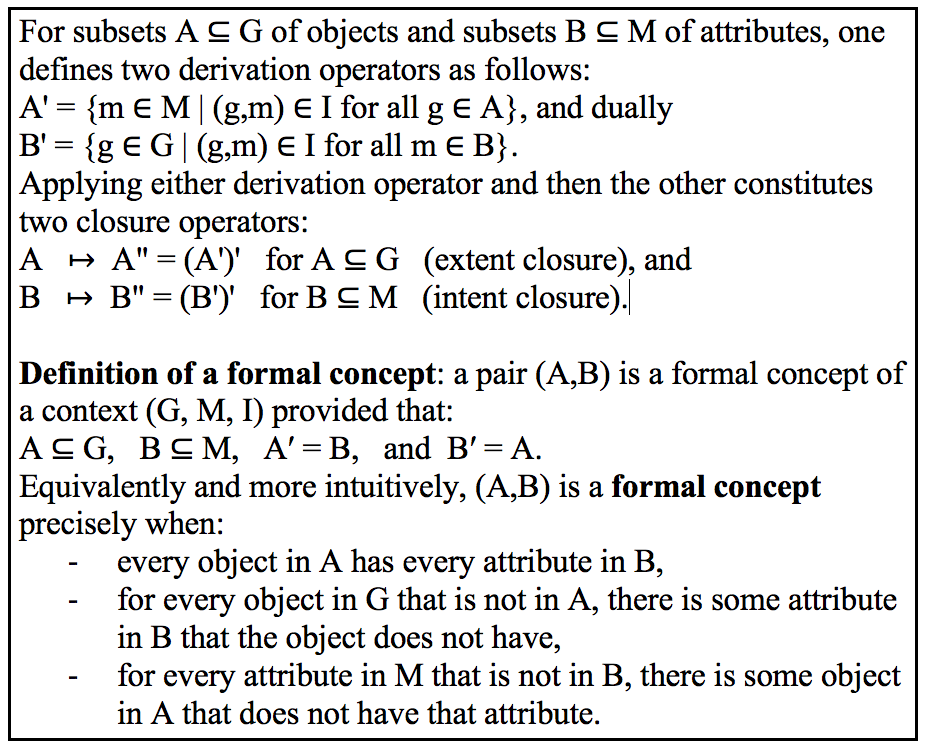
\includegraphics[width=0.45\textwidth]{figs/formalConceptDefinition.png}
\label{fig:formalConceptDefinition}
\end{figure}

A \textit{concept lattice} can be derived from a \textit{formal context} by specifying \textit{formal concepts} (Figure \ref{fig:formalConceptDefinition}) and a \textit{partial order} on them. Concept lattices are represented as a directed acyclic graph where concepts are nodes and the order on them determines the edges.
%
Figure \ref{fig:sampleCL} shows the concept lattice derived from the formal context in Table \ref{tab:sampleContext} and is interpreted as follows:

\begin{itemize}
    \item The top node indicates that all traces share MPI\_Init(), MPI\_Comm\_size(), MPI\_Comm\_rank() and MPI\_Finalize().
    \item The bottom node signifies that none of the traces share all attributes. 
    \item The middle nodes show that $T_0$ and $T_2$ are different from  $T_1$ and $T_3$.
\end{itemize}


\begin{table}[]
\label{tab:sampleContext}
\caption{Context}
\scalebox{0.6}{
\begin{tabular}{l|cccccc}
 & \multicolumn{1}{l}{MPI\_Init()} & \multicolumn{1}{l}{MPI\_Comm\_Size()} & \multicolumn{1}{l}{MPI\_Comm\_Rank()} & \multicolumn{1}{l}{MPI\_Send()} & \multicolumn{1}{l}{MPI\_Recv()} & \multicolumn{1}{l}{MPI\_Finalize()} \\ \hline
Rank 0 & $\times$ & $\times$ & $\times$ &  & $\times$ & $\times$ \\
Rank 1 & $\times$ & $\times$ & $\times$ & $\times$ &  & $\times$ \\
Rank 2 & $\times$ & $\times$ & $\times$ & $\times$ &  & $\times$ \\
Rank 3 & $\times$ & $\times$ & $\times$ & $\times$ &  & $\times$
\end{tabular}}
\end{table}


Once the redundant labels are removed from the lattice, each object (trace) and attribute appears in the lattice exactly once. Consequently, the nodes of the lattice form the desired grouping, since it is guaranteed that each trace belongs to exactly one group. However, the concept lattice itself does not provide similarity values for the distinct groups of traces. The \textit{Jaccard Index}, also known as \textit{Intersection over Union}, measures the \textit{distance} between sets $A$ and $B$ in terms of the ratio of the \textit{intersection} size of $A$ and $B$ over the size of their \textit{union}.  The complete pairwise Jaccard Similarity Matrix (JSM) can easily be computed from the concept lattice.
%


\begin{figure}[t]
\centering
\scalebox{0.5}{
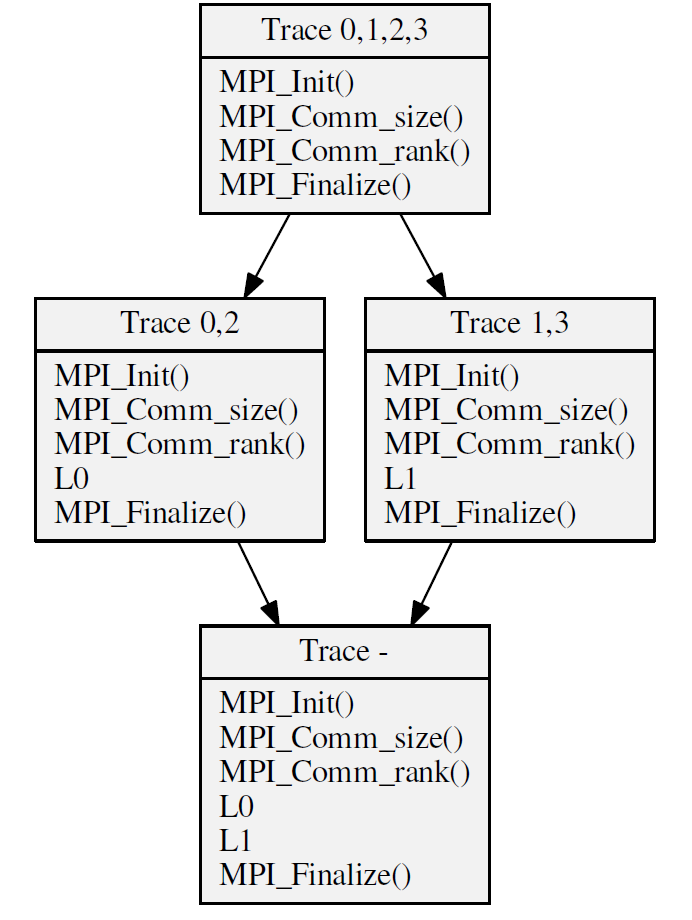
\includegraphics[width=3.4in]{figs/sampleCL.png}}
\caption{Sample Concept Lattice from Obj-Atr Context in Table \ref{tab:sampleContext}}
\label{fig:sampleCL}
\end{figure}


%\begin{figure}[]
%\centering
%\scalebox{0.8}{
%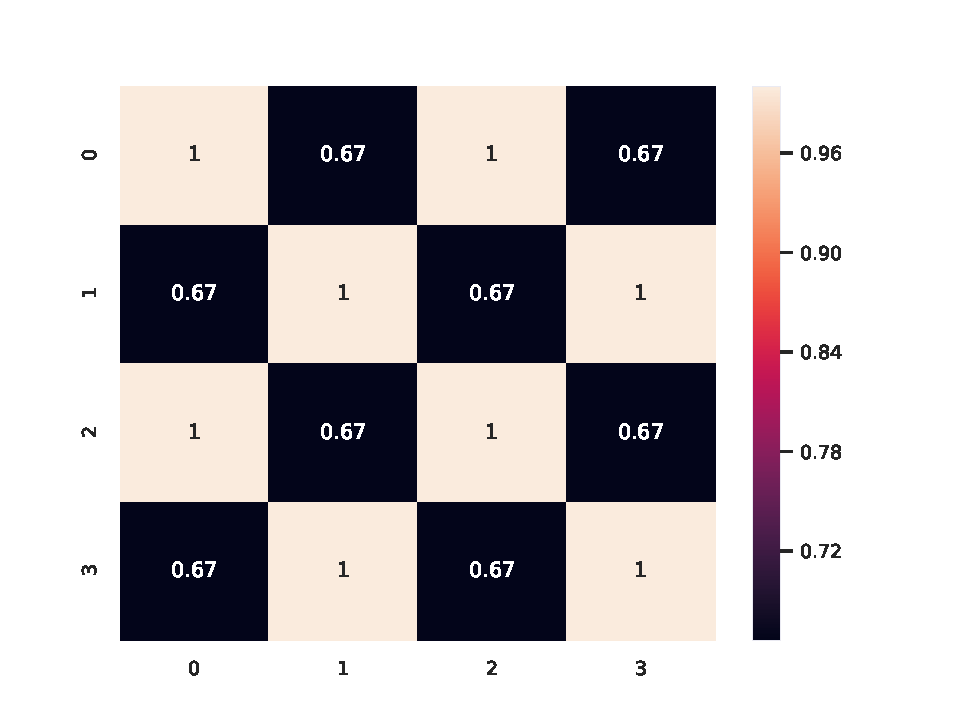
\includegraphics[width=3.4in]{figs/oddEvenJSM.pdf}}
%\caption{Pairwise Jaccard Similarity Matrix (JSM) of MPI processes in sample code}
%\label{fig:jsm}
%\end{figure}

\begin{figure}[]
\centering
\scalebox{0.8}{
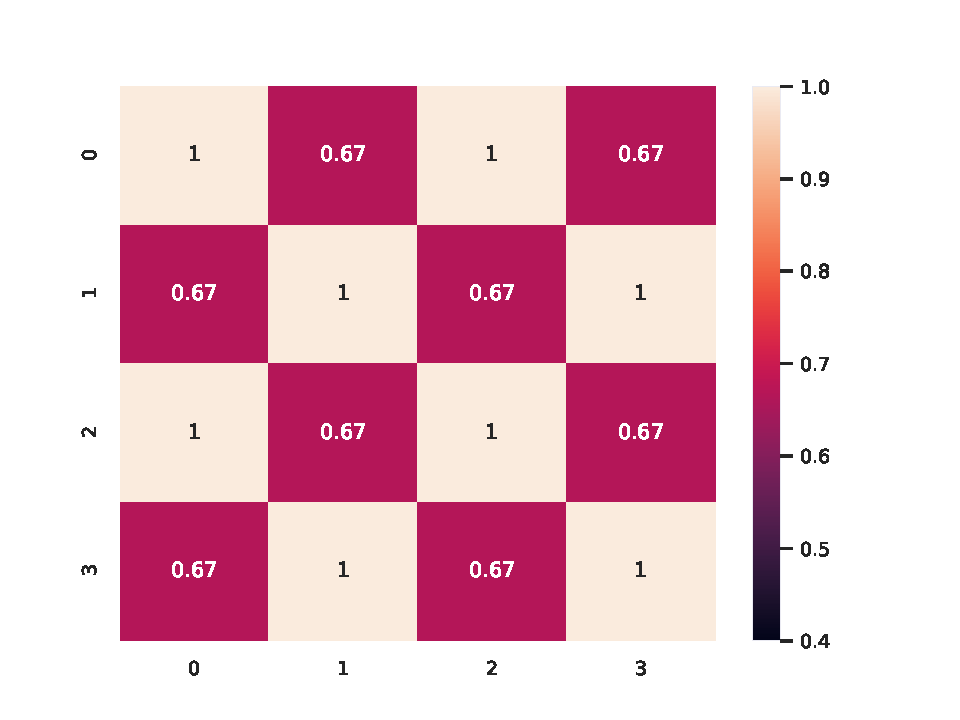
\includegraphics[width=3.4in]{figs/oddEvenJSM2.pdf}}
\caption{Pairwise Jaccard Similarity Matrix (JSM) of MPI processes in sample code}
\label{fig:jsm2}
\end{figure}

For any pair of $(T_i, T_j)$, the number of attributes in the Lowest Common Ancestor (LCA) node of $T_i$ and $T_j$ in the lattice is the number of attributes that $T_i$ and $T_j$ have in common (intersection). The sum of the number of attributes of the nodes on the path from each $T_i$ and $T_j$ to their LCA is the union. This property is one of the motivations for using concept lattices as classifier since it makes computing the union and intersection easy and fast.

Some algorithms for extracting concepts from contexts and constructing the concept lattice require the whole context to be present in the memory.
%
For large-scale executions with thousands of threads, this is not feasible.
%
Through an incremental concept-lattice-construction approach, DiffTrace extracts attributes (\hl{table that shows attributes}) from NLR traces and injects them into a concept lattice one trace at a time (cf. Section \ref{subsec:algo-cl}).
%
Figure \ref{fig:jsm2} shows the heatmap (explain this) of the JSM obtained from the concept lattice in Figure \ref{fig:sampleCL}.
%
DiffTrace uses the JSM to form equivalence classes of traces by hierarchical clustering.
%
Next, we show how the differences between two hierarchical clusterings from two executions (faulty vs.~normal) reveal which traces have been affected the most by the fault.


\subsection{Detecting Suspicious Traces via DiffJSM}
So far, we have explained how DiffTrace can narrow down the search space from numerous long traces to just a few equivalent JSMs (i.e., clusters).
%
$JSM_{normal}[i][j]$ ($JSM_{faulty}[i][j]$) shows the Jaccard similarity score of $T_i$ and $T_j$ from the normal trace ($T_i^\prime$ and $T_j^\prime$).

However, we are interested in detecting what changed the most due to the fault.
% with respect to the ``natural asymmetry'' of the application.
%
%In other words, DiffTrace abstracts function call traces into JSMs, which are reflections of asymmetry among traces.
The hierarchical clustering based on \textit{DiffJSM}, followed by the subtraction of the faulty JSM from its corresponding normal JSM, typically puts the trace(s) that changed the most in a separate, often singleton, cluster and thus detects the outlier.

$DiffJSM = |JSM_{faulty} - JSM_{normal}|$

% 
The resulting outlier traces are candidates for the potential cause of the change in the program behavior and thus a potential fault root cause or fault manifestation.
%
However, a single iteration of DiffTrace (with a single set of parameters shown as a dashed box in Figure \ref{fig.diffTraceOverview}) may not detect the problem. 
%
%Also, a different set of parameters might produce inaccurate suggestions (false positives).
%
To improve the accuracy, we have sorted the suggestion table based on the \textit{B-score} similarity metric of two hierarchical clusterings \cite{fowlkes83} (cf.~Section \ref{subsec:algo-bscore}).

To evaluate the effectiveness of DiffJSM, we planted two artificial bugs (\textit{swapBug} and \textit{dlBug}) in the code from Figure \ref{fig.oddEven} and ran it with 16 processes.
%
\textit{swapBug} swaps the order of MPI\_Send and MPI\_Recv in rank 5 after the seventh iteration of the loop in line 3 of \texttt{oddEvenSort}, simulating a potential deadlock. \textit{dlBug} simulates an actual deadlock in the same location (rank 5 after the seventh iteration).
%
Upon collection of ParLOT traces from the execution of the buggy code versions, DiffTrace first decompresses them and filters out all non-MPI functions.
Then two major loops are detected, \textbf{L0} and \textbf{L1} (Figure \ref{fig.gdiffs}-(a)), that are supposed to loop 16 times in the even and odd traces, respectively (except for the first and last traces, which loop just eight times).

After constructing concept lattices and their corresponding JSMs, trace 5 appears as the trace that got affected the most by the bugs because row 5 (showing the similarity score of $T_5$ relative to all other traces) ($JSM_{normal}[5][i]$ for $i \in [0,16)$) changed the most after the bug was introduced. %Consequently, it means that $T^\prime_5$ affected the asymmetry of all $T_i$s.
*
The differences between the suggested suspicious trace ($T^\prime_s$) and its corresponding normal trace ($T_s$) is visualized by \textit{diffNLR}.

\subsubsection{diffNLR}
To highlight the differences in an easy-to-understand manner, DiffTrace visually separates the common and different blocks of a pair of pre-processed traces via \textit{diffNLR}, a graphical visualization of the \texttt{diff} algorithm \cite{diff-myers}.
%

\begin{figure}[]
\centering
\caption{(a) The legend of \textit{diffNLR} and the list of loop structures (b) \textit{diffNLR(5)} of \textit{swapBug} (c) \textit{diffNLR(5)} of \textit{dlBug}}
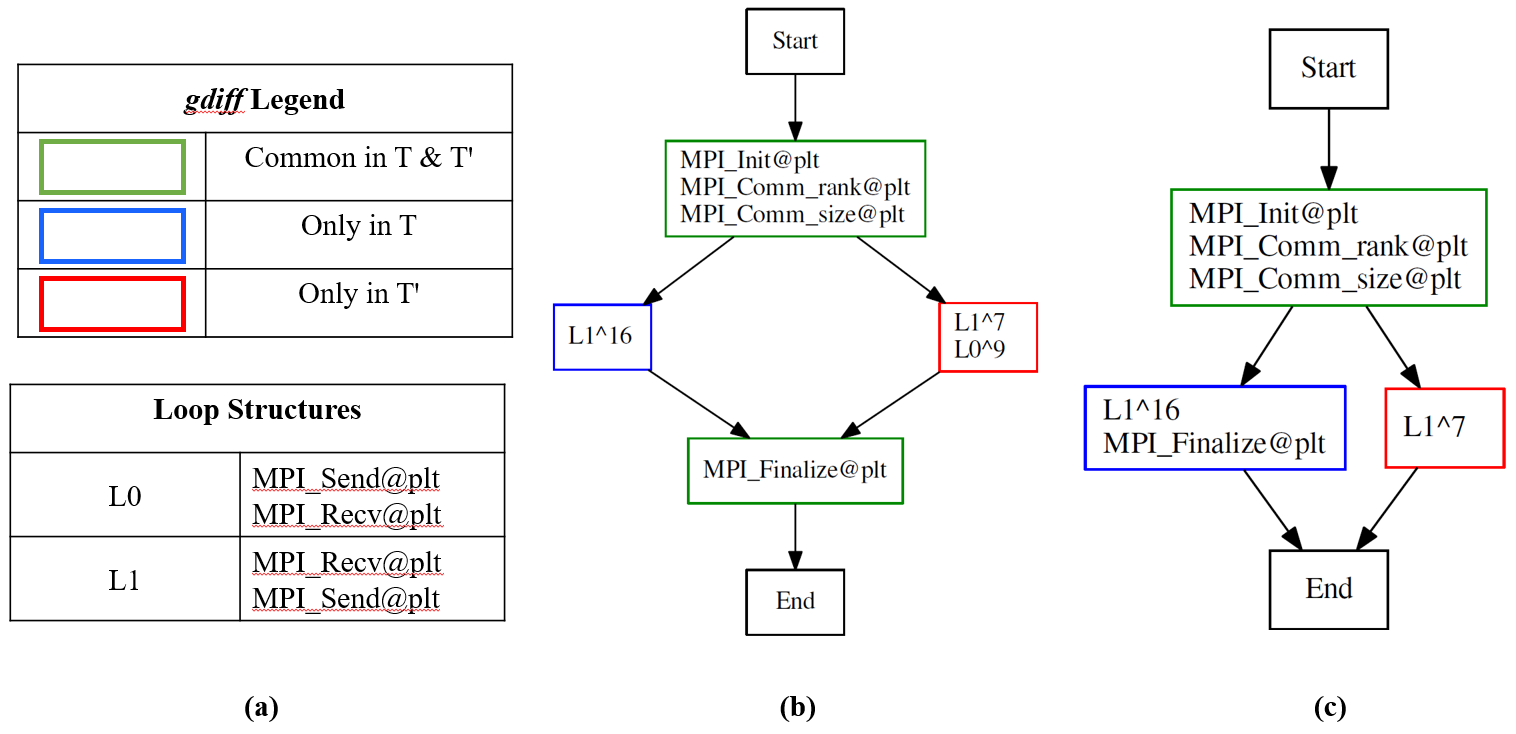
\includegraphics[width=0.45\textwidth]{figs/sampleGdiff.png}
\label{fig.gdiffs}
\end{figure}


\texttt{diff} takes two sequences $S_A$ and $S_B$ and computes the minimal \textit{edit} to convert $S_A$ to $S_B$. This algorithm is used in the GNU \texttt{diff} utility to compare two text files and in git for efficiently keeping track of file changes.
Since ParLOT preserves the order of function calls, each trace $T_i$ is totally ordered. Thus \textit{diff} can expose the differences of a pair of $T$s. \textit{diffNLR} aligns common and different blocks of a pair of sequences (e.g., traces) horizontally and vertically, making it easier for the analyst to see the differences at a glance.
For simplicity, our implementation of \textit{gdiff} only takes one argument $x$ that denotes \textit{the suspicious trace}.

diffNLR$(x) \equiv $ diffNKR$(T_x,T_x^\prime)$
%
where $T_x$ is the trace of thread/process $x$ of a normal execution and $T^\prime_x$ is the corresponding trace of the faulty execution.

Figure \ref{fig.gdiffs}-(b) shows the $diffNLR(5)$ of \textit{swapBug} where $T_5$ iterates over the loop [MPI\_Recv - MPI\_Send] 16 times (L1\^{}16) after the MPI initialization while the order swap is well reflected in $T_5^\prime$ (L1\^{}7 - L0\^{}9). Both processes seem to terminate fine by executing MPI\_Finalize(). 
However, $diffNLR(5)$ of \textit{dlBug} (Figure \ref{fig.gdiffs}-(c)) shows that, while $T_5$ executed MPI\_Finalize, $T_5^\prime$ got stuck after executing L1 seven times and never reached MPI\_Finalize.

This example illustrates how our approach can locate the part of each execution that was impacted by a fault. Having an understanding of \textit{how the application should behave normally} can reduce the number of iterations by picking the right set of parameters sooner. 


%\begin{figure}[]
%\centering
%\caption{A line change in oddEvenSort (left) that might cause a deadlock in oddEvenSort\_DL (right)}
%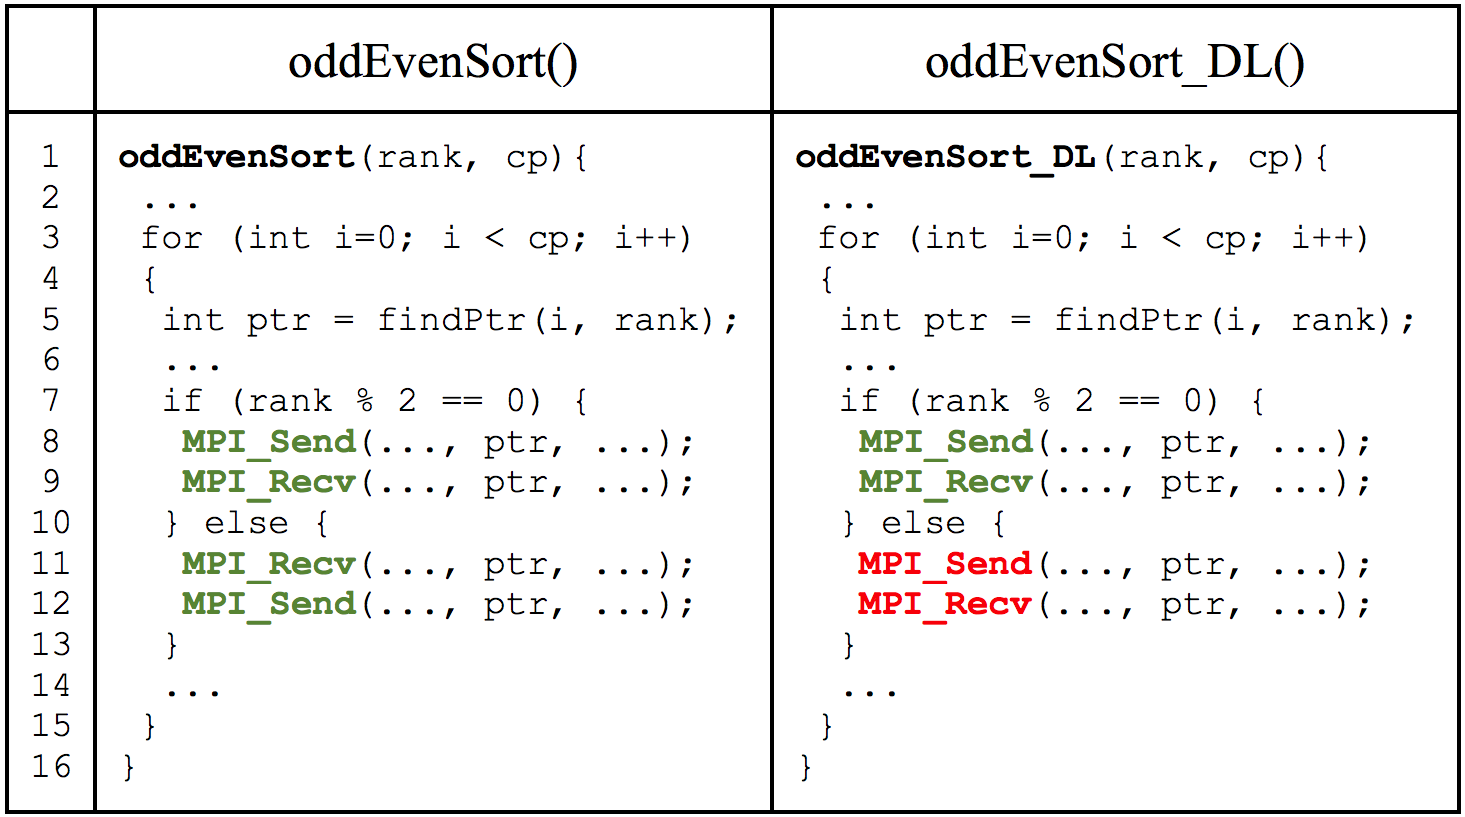
\includegraphics[width=0.45\textwidth]{figs/oddEvenDL.png}
%\label{fig.oddEvenDL}
%\end{figure}





